\documentclass{article}

\usepackage{parskip}
\usepackage[margin=1.6cm]{geometry}
\usepackage{amsmath,amssymb}
\usepackage{float}
\usepackage{graphicx}
\usepackage{subfig}
\usepackage{fancyhdr}
\pagestyle{fancy}
\usepackage{tcolorbox,listings}
\usepackage{color}
\usepackage{hyperref}
\usepackage{xcolor}
\usepackage{tikz}
\usepackage{babel}
\usepackage[babel=true,kerning=true]{microtype}
\usepackage{afterpage}
\usepackage{minted}
\definecolor{LightGray}{gray}{0.9}
\usepackage{multirow}

\newcommand\myemptypage{
    \null
    \thispagestyle{empty}
    \addtocounter{page}{-1}
    \newpage
}

\newminted[pythonCode]{python}{
    frame=lines,
    framesep=2mm,
    baselinestretch=1.2,
    bgcolor=LightGray,
    fontsize=\footnotesize,
    linenos}

\newminted[outputCode]{bash}{
    frame=lines,
    framesep=2mm,
    baselinestretch=1.2,
    bgcolor=LightGray,
    fontsize=\footnotesize,
    linenos}

\setlength{\headheight}{28pt}
\fancyhead[L]{Fabien ALLEMAND}
\fancyhead[C]{IA323 Computer Vision}
\fancyhead[R]{\includegraphics[scale=0.025]{/home/fabien/logo_TSP_1.jpg}}
\fancyfoot[L]{}
\fancyfoot[R]{}

\begin{document}

\begin{center}
    \baselineskip=25pt
    \textbf{{\Huge IA323 - Computer Vision}}\\
    \textbf{{\Large Practical Work: Fire Detection}}
\end{center}

\section{Introduction}
Classical approaches for image classification rely on deep neural networks trained on large datasets of images and labels, a technique called Supervised Learning (SL). Eventhough these methods have proven their worth for many image classification tasks, their supervised nature prevent them from being used in a wide variety of specific applications. Image labelisation is often time consuming and costly. For instance, simple tasks like object recognition require a lot of training samples to account for the variety of objects. In domains like medicine, experts are required to analyse data. It should also be noted that in both cases labelisation can be incorrect and negatively impact the training of the network. This is without mentioning the ethical issues hidden behind low income labelisation labour.

In this work, we try to reduce the use of labelised data by exploring Self-Supervised Learning (SSL) techniques that can leverage hidden knowledge contained in images without labels. The goal of this study is to assess the performance gain of SSL on downstream tasks that have large amount of unlabeled data available but few labeled data. We apply this technique to wildfire detection through satellite images as analysing satellite images is a domain where SL would require experts to annotate large databases of images to the best of their ability. A process that end up being costly, time consuming and unreliable. First, we introduce the dataset and do a quick overview of self-supervised techniques. Then, we present our method and analyse the results.

\section{Wildfire Prediction Dataset}
Trhoughout this study, we use the Wildfire Prediction Dataset (Satellite Images)\footnote{\url{https://www.kaggle.com/datasets/abdelghaniaaba/wildfire-prediction-dataset/data}}. This dataset contains 42850 satellite images of areas that previously experienced wildfires and areas that did not. These images are \(350 \times 350\) pixels color images split in two classes: wildfire and no wild fire. Examples of images can be seen on Figure \ref{data}. This dataset is split into three subsets for training, validation and testing. Table \ref{tab_1} show that classes are balanced in all splits.

\noindent
\begin{minipage}[!hc]{0.12\textwidth}
    \begin{flushleft}
        \textbf{Note:}
    \end{flushleft}
\end{minipage}
\vrule\enskip\vrule\quad\begin{minipage}{\dimexpr 0.87\textwidth-0.8pt-1.5em}
    This dataset contains labels for all images. However, in this study, we do not use the labels of the train split.
\end{minipage}

\begin{figure}[]
    \centering
    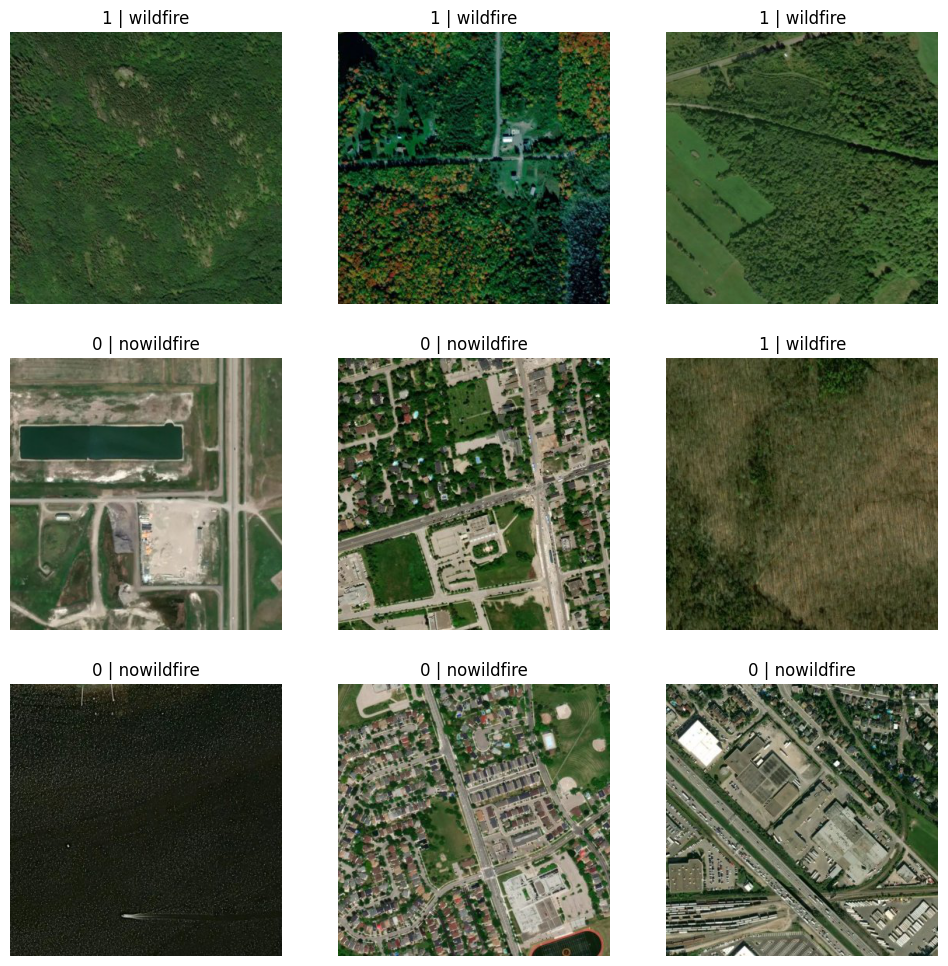
\includegraphics[width=10cm]{img/data.png}
    \caption{Visualisation of images from the Wildfire Prediction Dataset.}
    \label{data}
\end{figure}

\begin{table}[]
    \centering
    \begin{tabular}{|l|r|r|r|r|}
    \hline
    \multicolumn{1}{|c|}{Class} & \multicolumn{1}{c|}{Train split} & \multicolumn{1}{c|}{Validation split} & \multicolumn{1}{c|}{Test split} & \multicolumn{1}{c|}{Total} \\ \hline
    Wildfire                    & 15750                            & 3480                                  & 3479                            & 22709                      \\ \hline
    No Wildfire                 & 14499                            & 2820                                  & 2820                            & 22709                      \\ \hline
    Total                       & 30249                            & 6300                                  & 6299                            &                            \\ \hline
    \end{tabular}
    \caption{Number of samples in each class of the dataset. Two corrupted images had to be removed from the dataset.}
    \label{tab_1}
\end{table}

\section{Self-supervised Learning}
Self-supervised learning is a machine learning paradigm where the model is trained in two steps. First, there is an auxiliary or pretext task whose goal is to learn insights and capture essential features of the data itself. This task does not require labels and can be seen as initialising the weights of the neural networks in a way that suits the data. Next, the downstream task can be performed, in our case using SL with labelised data.

There are different types of SSL. In this work we use:
\begin{itemize}
    \item Contrastive: The goal of the pretext task is to minimize the distance between data that are known to be similar and maximise the distance between those that are different.
    \item Autoassociative: The auxiliary task consists in reconstucting the input data.
\end{itemize}

\section{Method}
Our work is based on the the SimCLR framework presented \textit{A Simple Framework for Contrastive Learning of Visual Representations}\footnote{\url{https://arxiv.org/abs/2002.05709}}. This framework apply contrastive SSL to images. The goal of the pretext class is thus to minimise the distance between similar images on the latent space while maximising the distance between different images. Figure \ref{simclr}, represents the framework for the pretext task. For each batch of data, each image \(x\) undergo two different transformations in order to create a positive pair. The goal of the neural network is to project these two transformed images close together in the latent space but far from all other images in the batch (considered as negative pairs).

\begin{figure}[]
    \centering
    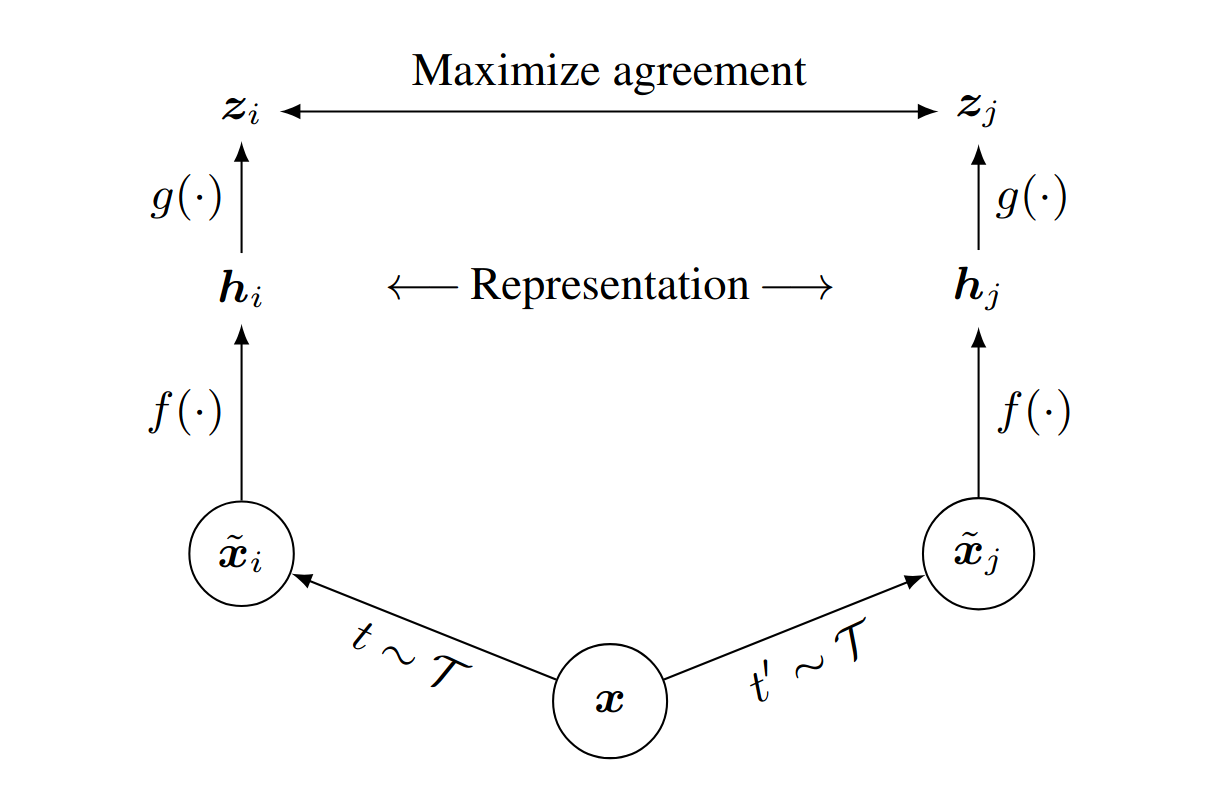
\includegraphics[width=10cm]{img/simclr.png}
    \caption{SimCLR framework.}
    \label{simclr}
\end{figure}

For all experiments the data used for the pretext task is the training split of the Wildfire Prediction Dataset (using only the images). We then use a portion of the validation split for training our neural network on the downstream task, in our case the image classification.

As recommanded when using the SimCLR framework, the transformation to create positive pairs consists of randomised resized crop, randomised flip (horizontal and vertical), randomised color distortion and randomised Gaussian blur. Examples of images and their transformation are presented in Figure \ref{transform}.

\begin{figure}[]
    \centering
    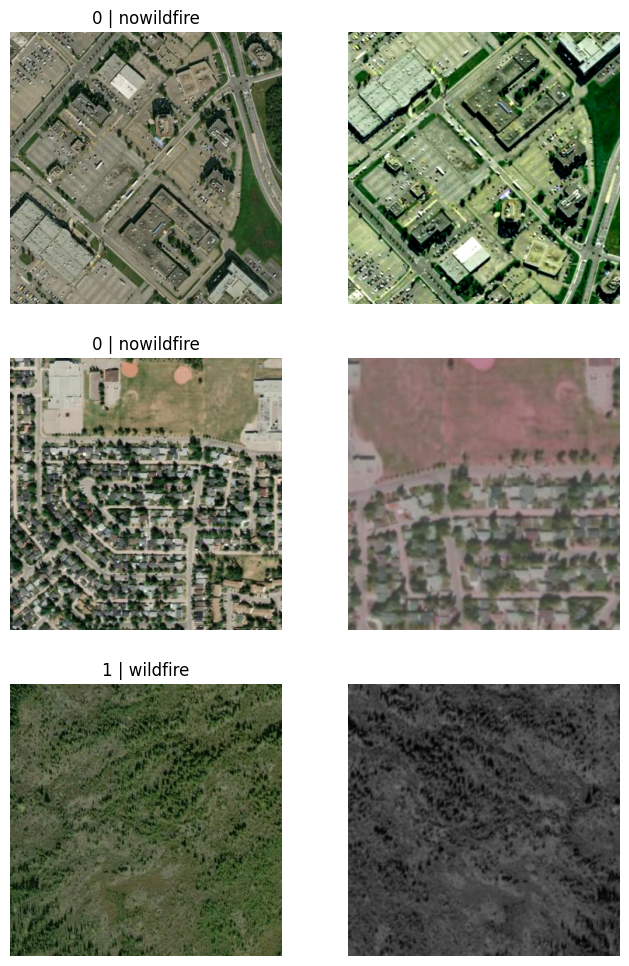
\includegraphics[width=10cm]{img/transform.png}
    \caption{Visualisation of images from the Wildfire Prediction Dataset before and after transformation.}
    \label{transform}
\end{figure}

For the pretext task, we use a ResNet-18 with two dense layers with ReLU activation function to project data in a 128 dimensions latent space. We train the for 100 epochs. Once the auxiliary training is complete, we freeze the encoder and change the head on the neural network (three dense layers with ReLU activation) to train the neural network for binary classification during 50 epochs.

We also perform some autoassociative SSL experiments with a UNet neural network. The UNet is trained for 100 epochs to reconstruct images. We then keep only the encoder and add a three layers head to perform binary classification and train again for 50 epochs with the encoder frozen.

We compare our downstream neural networks with similar ones trained only for the downstream classification task. That is to say neural networks that were not trained with any auxiliary task but only for classification with the same amount of data as our downstream neural networks. However, we use a pre-trained ResNet-18 encoder.

The goal of this study is to assess the performance gain of SSL on downstream tasks that have large amount of unlabeled data available but few labeled data, in our case, satellite images to predict past wildfires. Keeping the same encoder trained on the auxiliary task, we train different models for the downstream classification using different sizes of datasets. This way, we can evaluate to what extend large amount of unlabeled data can compensate for a lack labeled data.

\section{Results}
First and foremost, Figures \ref{resnet_m} and \ref{unet_m} show that all models achieve reasonably good performance on the classification task. The accuray is always above 0.9. As expected, the amount of data used for supervised training impact performance. For both ResNet and UNet based classifiers, the accuracy and F1-score increase with the number of training samples.

Interestingly but unsurprisingly, the models trained with SSL are more preformant than their supervised counter part. In Figures \ref{resnet_m} and \ref{unet_m}, self-supervised models are consistantly above supervised models in both accuracy and F1-score. What is definitly interesting is how this performance gap evolves with the number of training samples. The less training samples the larger the gap. This means that self-supervised trained neural networks benefit from the auxiliary training and are less impacted by the lack of labelised data.

\begin{figure}[]
    \centering
    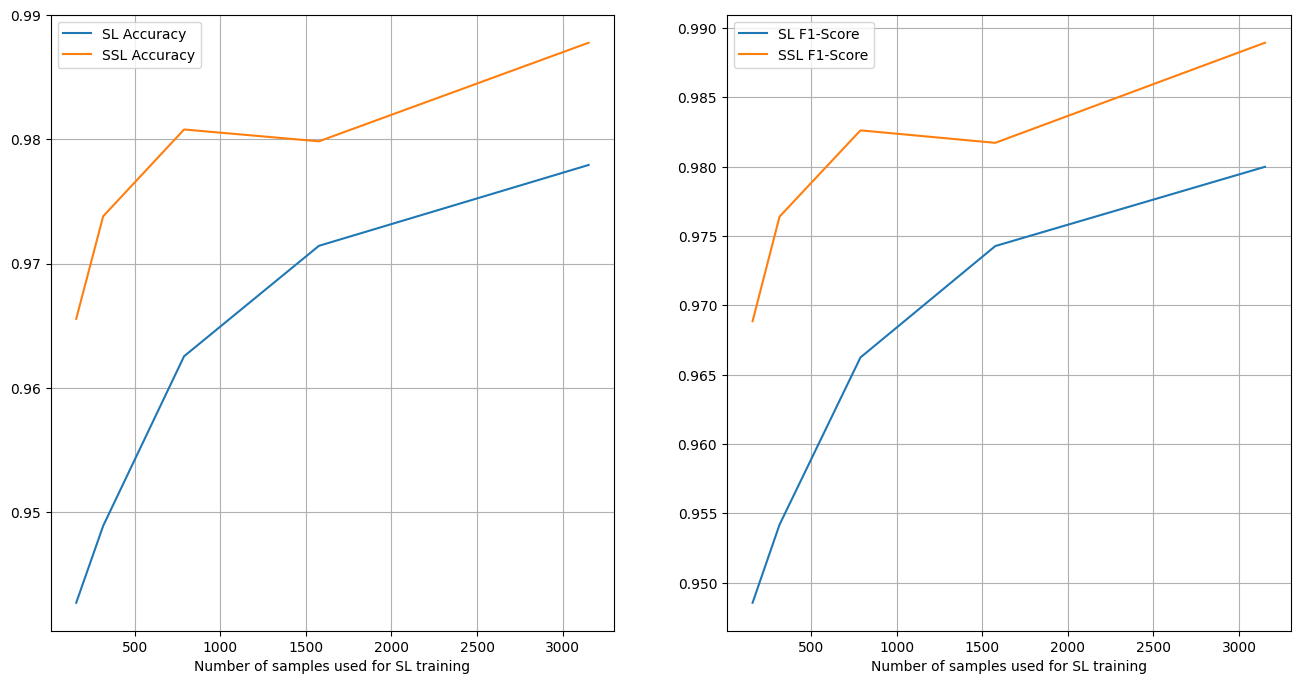
\includegraphics[width=15cm]{img/resnet.png}
    \caption{ResNet based classifier classification performance based on training samples.}
    \label{resnet_m}
\end{figure}

\begin{figure}[]
    \centering
    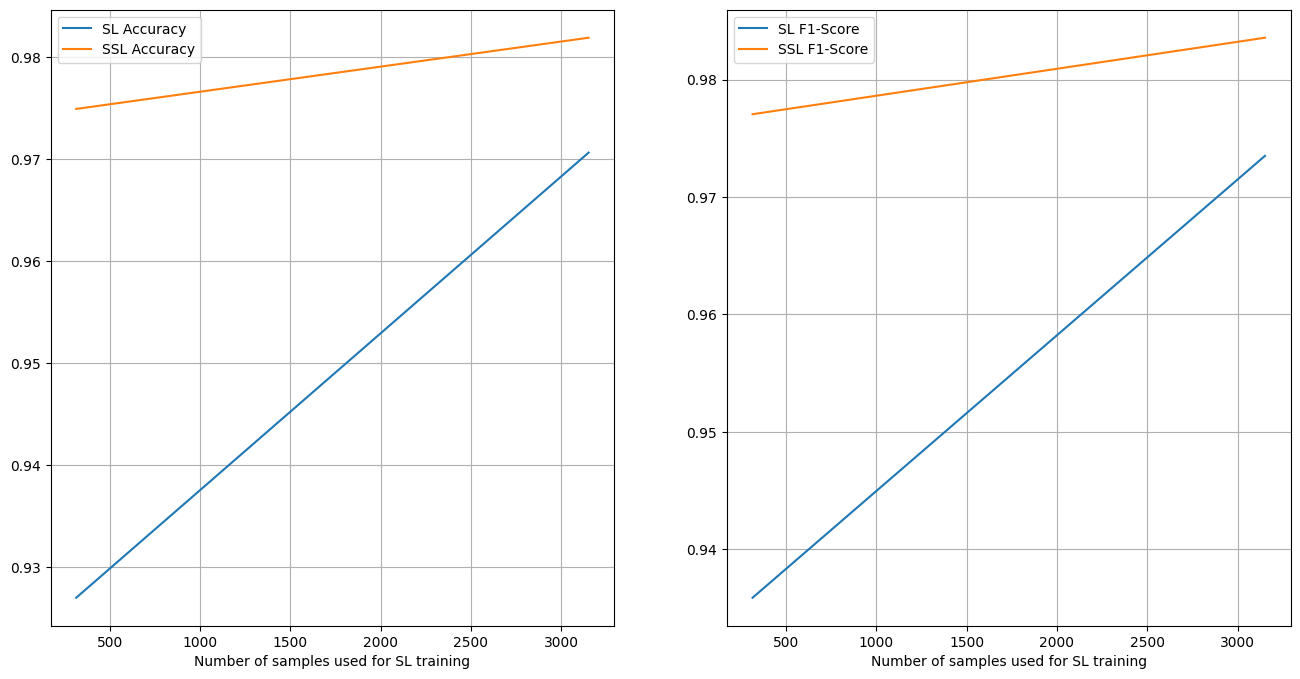
\includegraphics[width=15cm]{img/unet.png}
    \caption{UNet based classifier classification performance based on training samples.}
    \label{unet_m}
\end{figure}

In this paragraph, let us imagine we worked on a different task such as predicting current wildfires through real time satellites images. With wildfire prediction, false positive but mostly false negative can have important consequences. The former can lead to wasting firefighters resources, the latter to disastrous losses. Figure \ref{resnet_conf} show that with only 160 labeled training samples, both SL and SSL models perform similarly. There is no model that is clearly better in one way or another (preventing useless actions or avoiding fires). 

\begin{figure}[H]
    \centering
    \subfloat[SL]{{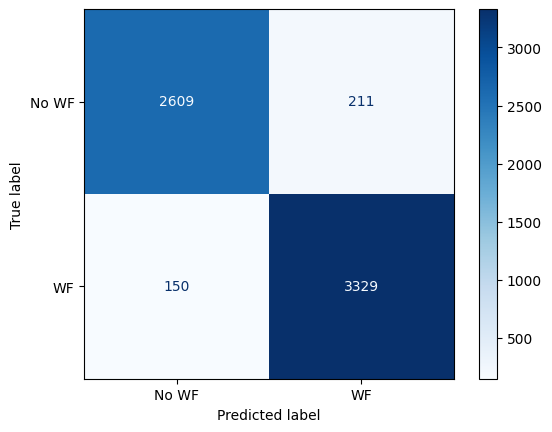
\includegraphics[width=7.5cm]{img/sl_conf.png} \label{resnet_conf:a}}}
    \qquad
    \subfloat[SSL]{{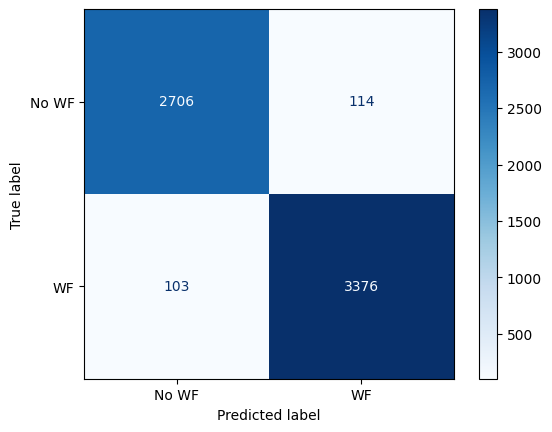
\includegraphics[width=7.5cm]{img/ssl_conf.png} \label{resnet_conf:b}}}
    \caption{Confusion matrices for classification task with ResNet based classifiers trained with 160 labeled samples.}
    \label{resnet_conf}
\end{figure}

It is also interesting to notice that SL and SSL models do not classify images based on the same criteria. Figure \ref{resnet_gradcam} show visual explanation of classification using GradCAM. Both neural networks use different features to classify. This is noticeable in Figures \ref{resnet_gradcam:b} and \ref{resnet_gradcam:c}

\begin{figure}[H]
    \centering
    \subfloat[No wildfire sample]{{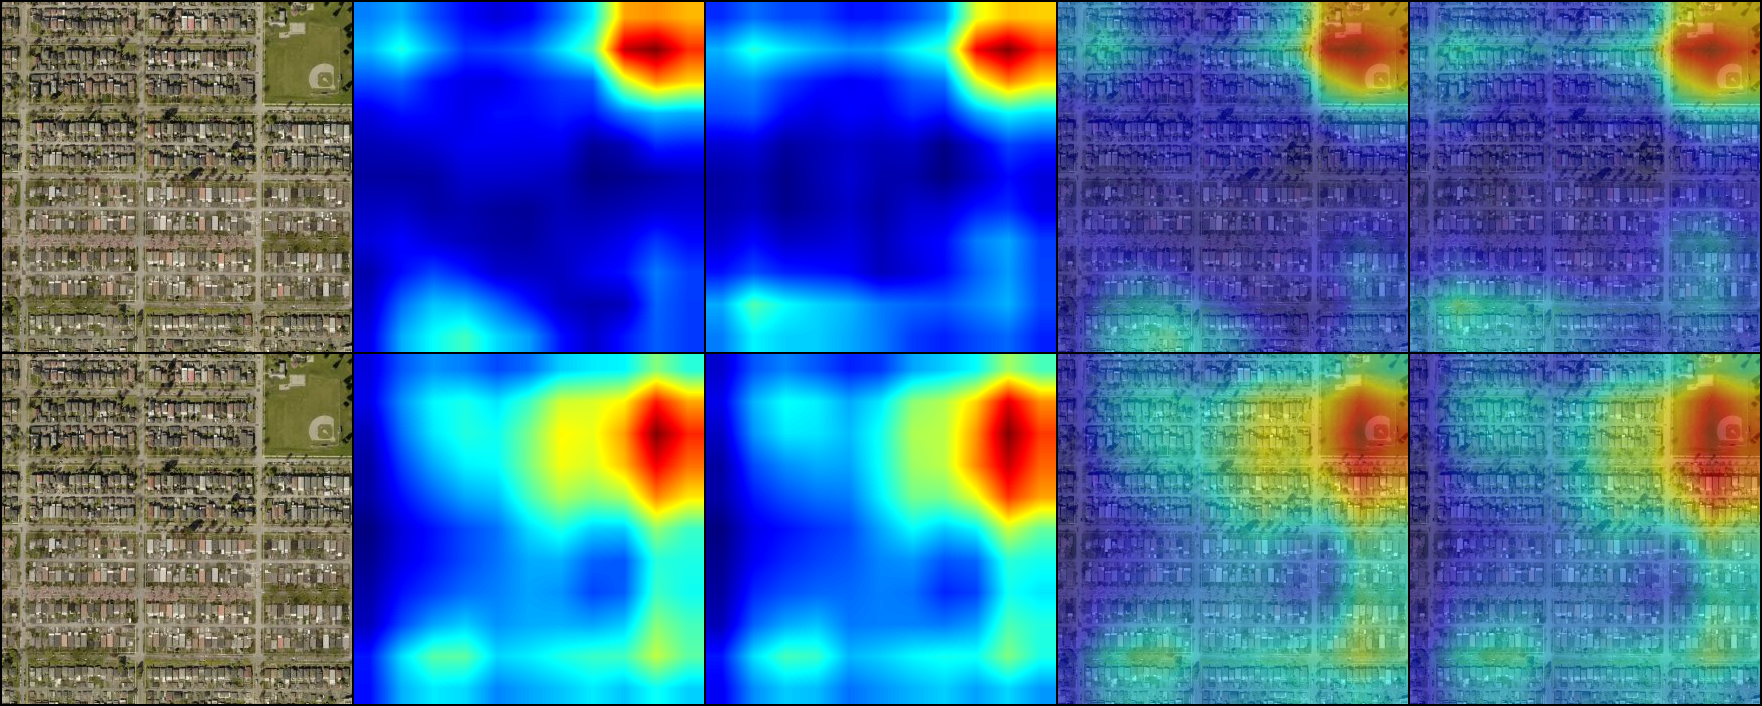
\includegraphics[width=15cm]{img/gradcam_nwf.png} \label{resnet_gradcam:a}}}
    \\
    \subfloat[Wildfire sample]{{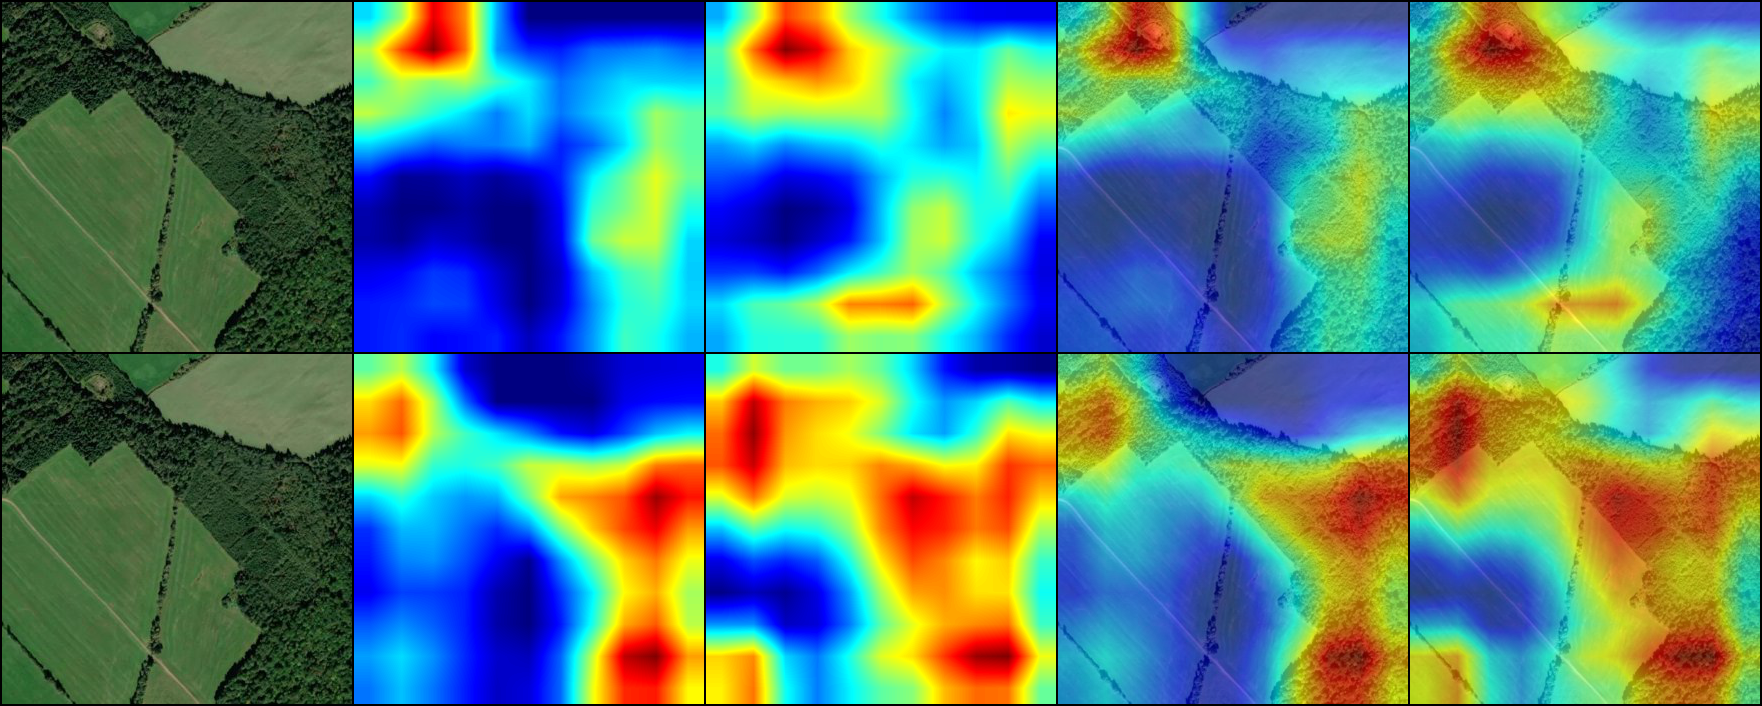
\includegraphics[width=15cm]{img/gradcam_wf_1.png} \label{resnet_gradcam:b}}}
    \\
    \subfloat[Wildfire sample]{{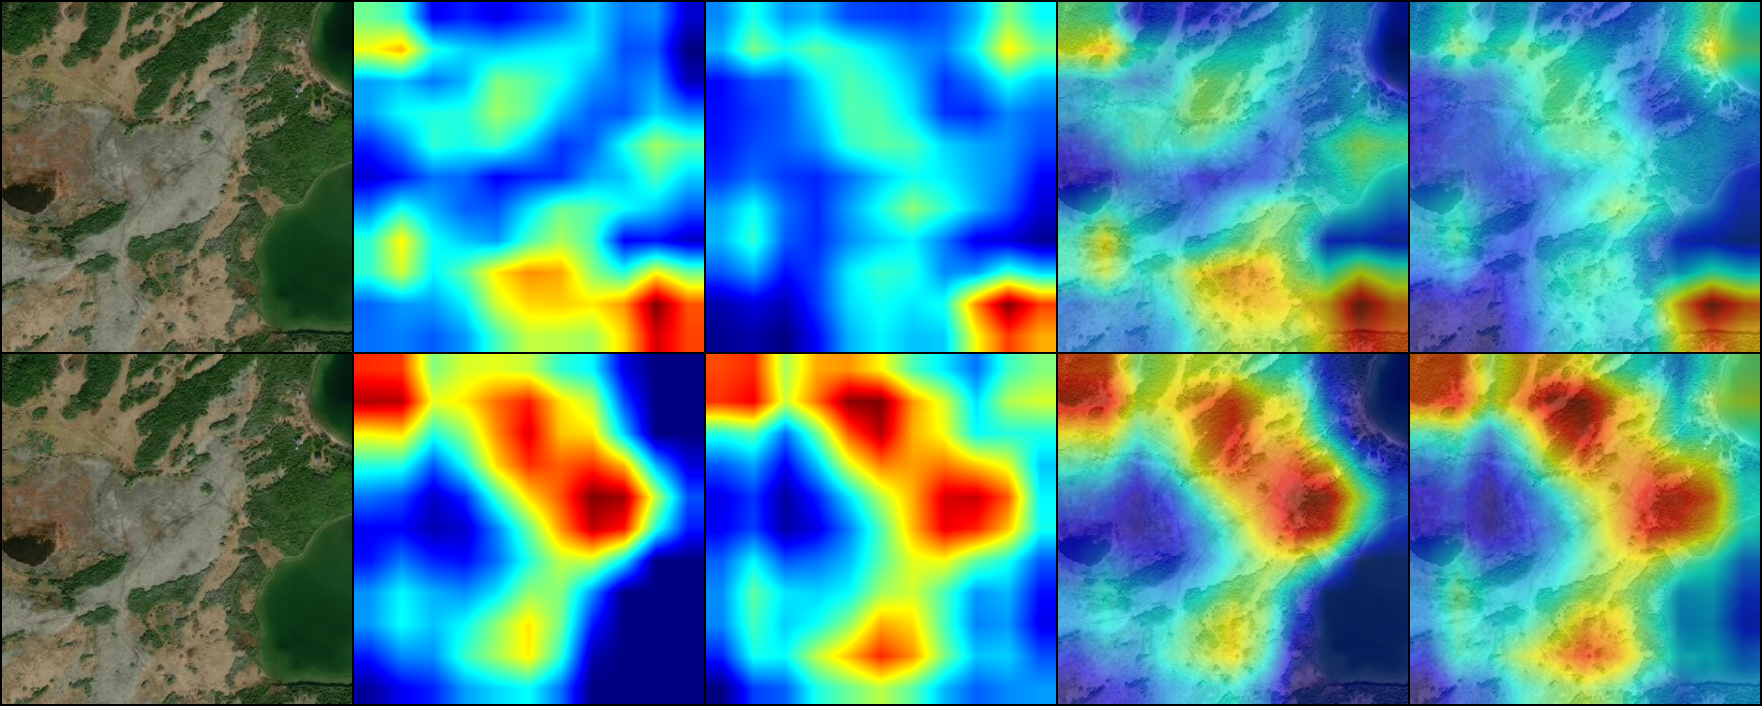
\includegraphics[width=15cm]{img/gradcam_wf_2.png} \label{resnet_gradcam:c}}}
    \caption{Visual explanation of classification on ResNet based classifier using GradCAM (top row: SL neural network, bottom row: SSL neural network).}
    \label{resnet_gradcam}
\end{figure}

\section{Conclusion}
Many possible classification tasks suffer from a lack of high quality labelised data due to cost and time constrains. Self-supervised learning is a machine learning paradigm that laverage insights contained into unlabeled data through an auxiliary task before performing the downstream task. The goal of this study was to assess the performance gain of SSL on downstream tasks that have large amount of unlabeled data available but few labeled data. We focused on satellite images to predict areas that experienced wildfires and found that SSL can indeed compensate for a lack of labeled data. Despite being considerable, it should however be mentioned that the gain was not enormous. Partly due to the fact that the neural networks with SL training only always achieved great performance. As pointed out by Kaggle users\footnote{\url{https://www.kaggle.com/datasets/abdelghaniaaba/wildfire-prediction-dataset/discussion/436007}}, the dataset could contain biased data that induce neural networks to do the wildfire classification based on other criteria such as rural/urban areas which would dramatically simplify the task. We performed quick experiments (notably GradCAM analysis, Figure \ref{resnet_gradcam}) and found no clear demonstration of such bias but further experiments should be carried out.

\end{document}